\documentclass[12pt]{article} %12pt font and article style

\usepackage{graphicx} %to import pictures if necessary
\graphicspath{ {images/} }
\usepackage{amsmath} %to allow math symbols to show up
\usepackage{fullpage}

\begin{document}
\begin{titlepage}
%I 'borrowed' this title page example from: https://en.wikibooks.org/wiki/LaTeX/Title_Creation
\centering
    {\scshape\LARGE University of Prince Edward Island\par}
    \vspace{1cm}
    {\scshape\Large Honours Thesis\par}
    \vspace{1.5cm}
    {\huge\bfseries Fashion Forward-Propagation: Machine Learning Tackles Fashion Curation\par}
    \vspace{2cm}
    {\Large\itshape Hailey LeClair\par}
    \vfill
    supervised by\par
    Dr.~Andrew \textsc{Godbout}

\vfill

\today\par

\end{titlepage}


\section{Introduction}


	When we see someone wearing a really nice pair of shoes, wouldn't it be nice if we could just take a photo or their shoes, and have some third party tell us where these shoes came from? My project will attempt to do this by using convolutional neural networks trained on specific clothing items that will try to find a match to the photo that is input. Over the past twenty years or so, the fields of computer vision and machine learning have been able to come up with innovative ways to detect and classify many different kinds of objects in images. Most rigid objects like boxes, pens, and even shoes can be detected in an image and a neural network can be trained classify a box as a box, or a shoe as a shoe. This kind of image recognition and classification seems seems to work very well for rigid objects, but what about deformable objects? If I take a photo of a dress on a woman, and want to find an image of the same dress online, what if the women wearing the dresses have completely different body shapes? What if in one photo the dress is blowing in the wind and one is not? This paper will look at these questions, and see if and how they can be answered. 
	
\section{Objects in Images}

	Rigid, articulated, and deformable objects all need to be considered when doing object detection, recognition, or classification in images. A rigid object (or body) is one that where, in terms of physics, "The distance between any two given points on a rigid body remains constant in time regardless of external forces exerted on it "\cite{RigidBodyWiki}. In terms of images, this means that the rigid object will always have the same dimensions, or some translation of the same dimensions in any photo taken of this object. Articulated objects are ones that may have rigid parts, but like human body parts, are connected at a joint which can move\cite{szeliski2010computer}. Multiple images of the same articulated object may show the object in different formations or positions. Although parts of these objects are rigid, possible movements from the joints, mean that there are many different positions each rigid part of an articulated object could take on. A deformable object is one that "changes its shape and/or volume while being acted upon by any kind of external force"\cite{wolfram}. Depending on the degree to which an object deforms, or the amount of force applied, many images of an object could show it as having completely different dimensions and shape. 
	
\section{PUT A FIGURE OF ARTICULATED RIGID AND DEFORMABLE OBJECTS HERE}
	
	
	The idea here is to take an image, classify it and find its' match amongst a set of similar photos, which means we need to be able to recognize the object in another image. There 	exist many methods to recognize rigid objects in an image, like SIFT (Scale Invariant Feature Transform). SIFT can recognize any object that doesn't vary in images based on image rotation, scaling, or translation. It also does well with different illumination and 3D projection \cite{lowe1999object}. Since rigid objects often have the same shape or dimensions in any image, edge detection methods can also be a good starting point to recognizing an object amongst noise in an image. It is great that that we can use methods like SIFT or edge detection to recognize a rigid object in an image, but what about articulated and deformable objects? 

	With a few exceptions(shoes, jewelry, accessories, etc.), most clothing items are deformable to a degree. For instance, a pair of skinny jeans may have a general shape on a hanger, but will have different dimensions and possibly even a different shape on different people. Like jeans, many clothing items take on the shape of the person wearing them. We cannot rely on something like SIFT\cite{lowe1999object} to recognize these sorts of items in an image. Usually, in images, clothing items are being worn by someone. This simple fact adds an extra dimension to recognizing the clothing item itself because the human body is an articulated body. Different articulations of the joints in the human body (especially our knees, shoulders, and elbows) can dramatically effect the shape and dimensions of a clothing item in an image. A loose denim jacket, which has a similar shape on anyone who wears it can be easily deformed by placing the arms in a different position. These obstacles specific to clothing items add a layer to object recognition for clothing items that is not present in recognizing many other types of objects in images.

\begin{figure}[h]
%\centering
%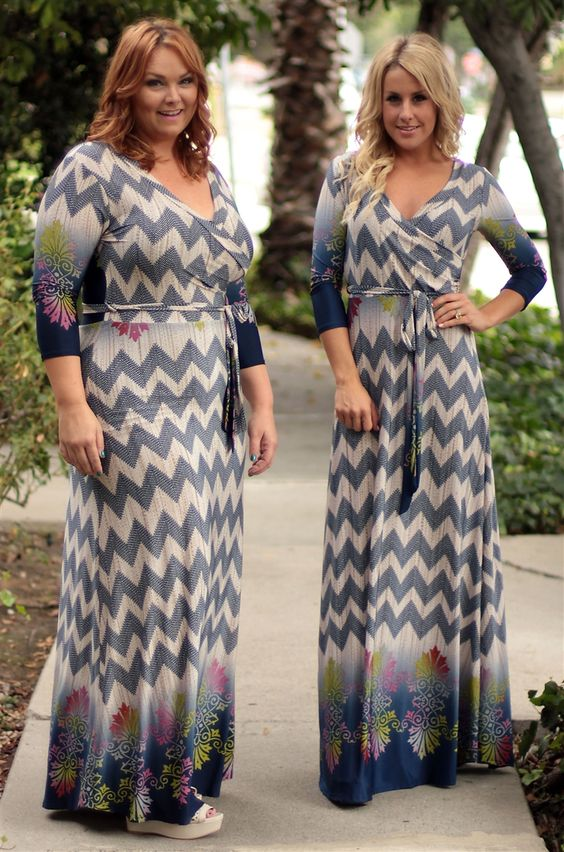
\includegraphics{dress_difference} 
\caption{The same dress on two different women with different shaped bodies}\label{fig: 2}
\end{figure}

	Along with the problem of objects being deformable and on an articulated body, we also have to consider other parts of an image. As intelligent humans, we can easily see if a dress in an image is the same as another dress in another image regardless of what other objects are in the background.  An image containing a clothing item could be convoluted with other objects or people in it, or could have an obvious plain background. A method that is able to recognize and classify these objects must account for these degrees of freedom that come with this task. For instance, if we have the same object in multiple images with a white background, a computer may then recognize the white background as a defining feature of this image. When introduced to another image of the same object with a noisy background a computer may then think this is a different object because of the dramatic different in backgrounds amongst this photo and the previous one(s). 
	
 \section{PUT A PICTURE OF A  VERY CONVOLUTED IMAGE HERE }

	The angle that a photo was taken and the location of a particular item in the image is also an important consideration. All known images of an object could be front-facing and if a side view of this object is introduced a computer will have nothing similar to this side view. In this case, the computer will not be able to correctly classify or recognize this object since it has no previous knowledge of its' side view. When they are being worn, clothing items like shoes and hats are almost always near the bottom and top of an image respectively. If a computer has only seen images of shoes in which they are located near the bottom edge of the image, a computer may think that this location is a common characteristic of shoes themselves. This must be considered when choosing images for a computer to classify or match. A shoe can be anywhere in an image and recognizing this when choosing images lets the focus be on features of the object itself. 
	
	Even if articulation, deformability, angle and rotation have all been taken into consideration when attempting to classify and recognize objects, colour and illumination must also be added to this long list of considerations. Depending on the lighting conditions and camera, the same red shirt may look pink in one image and orange in another. An image must be recognizable under different lighting conditions or minor variations in the object's colour. What if an image of this shirt is greyscale? This is an important question. If the goal is to recognize a red shirt in an image, greyscale images must not be considered. If they are considered they must be accepted as either grey or colourless even if the shirt in the image is actually red, in this case, the greyscale image is irrelevant. If the goal is to recognize a plain shirt, colour becomes unimportant and a greyscale image is as relevant as an RGB image.
	
 \section{PUT A PICTURE OF A SHIRT IN COMPLETELY DIFFERENT LIGHTING}
	
	When recognizing clothing items in images, it is almost impossible to account for every possible variant from image to image. However, if we keep all of these degrees in freedom in mind when attempting to classify or match images, we can avoid many of the problems that come with these variations. Where do we start in terms of finding similarities in different images? Just one approach, but a good approach, is to find an identify features specific to a certain object in almost every image of the object. Viola and Jones did this in 2004 with Real-Time Robust Face Detection. They classified faces in images based on the computed values of simple features specific to faces.\cite{viola2004robust}. They used simple rectangles(figure of viola and jones rectangles) to find areas in brightness in a photo.If these areas of brightness are present, the image it contains a face. Viola and Jones' specific facial recognition only works on images of faces. Naturally, one would imagine that a similar process to this facial recognition could be used in attempting to recognize other objects in images, like clothing. In theory, we should be able to find prominent features that belong to each type of clothing item, and use this feature to classify the image.

%THIS IS A PARAGRAPH THAT HAS TO BE TAKEN APART	
	
	Multiple filters applied to the same image will give us multiple feature maps which can show us whether or not a specific feature is prominent in an image.\cite{aurelienMachineLearning}. If every image of a certain class in a training set is found to have a specific feature, a machine learning algorithm will use this feature to predict whether or not an image belongs to this class. For example, a filter that find horizontal lines in an image might be a good predictor of a pair of pants being present in an image. If it is found to be a good predictor by a machine learning algorithm, and horizontal lines are prominent in a new image, pants will be a considered class for this image. 
	
%ENDS HERE
		
	 As stated above, in images, we count on an item to have one or more identifying features, like a human face. One of the ways that we can find the parts in an image that are likely to be important, and make them more prominent is by applying a filter to the image. A common example of a filter is the use of a neighbourhood operator, or local operator on pixels in an image. A neighbourhood operator uses an area of pixels around a specific pixel in an image to give a compute an output value for that pixel. When applied to all pixels across an image, the operator "filters" the image. A neighbourhood operator takes a weighted sum of all pixels in a neighbourhood and is also known as a correlation. Where h(k, l) are called the filter coefficients. A variant on this operator is the convolutional operator which is both commutative and associative. The convolutional operator is a reversal in f of the sign of the offsets g = f * h where h is now an impulse response function.\cite{szeliski2010computer}. 

\[g(i,j) = \sum_{k,l} f(k, l)h(i + k, j + l)\]
%That's a convolutional operator
	
	Filters can be used for edge detection, to blur photos, to adjust colour, or to sharpen images.\cite{szeliski2010computer}. Filters can play a crucial part in detecting any object in an image as it makes it easier for a computer to recognize certain features in an image, but to manually find which features are important and which filters or convolution kernels work for each object is not a feasible task. Filters are helpful in discovering features in an image and making them more prominent, but with 1000 or more images how do we know which filters to use or what features are important? 
	
	Machine Learning can help us "learn" things about these images, like which filter and convolution kernels work best, without having to manually go through this process. Simply put, Machine learning is programming a computer to learn something from the data itself. People use machine learning to analyze and monitor data much more efficiently than doing it manually. It can be used to learn what people are buying, which emails in your inbox are spam, and in this case, if a pair of jeans is in an image, and which pair of jeans it is. \cite{aurelienMachineLearning}. Using machine learning algorithms, we can program a computer to learn about almost anything as long as we provide it with enough data, and the right data. For instance, If we want a computer to use machine learning to "learn" if a pair of shoes are present in an image, we have to make sure we provide it with many images of many different kinds and brands of shoes. These images are called our training set.\cite{aurelienMachineLearning}. The images in the training set are input into a machine learning algorithm. The algorithm then goes through the entire set of images and looks for similar features among all or most of the images. 
	
	The first step in this process of matching objects in images is to recognize (or correctly classify) a clothing item in an image. A machine learning algorithm needs to learn the way in which it will get the best results with the information available. This information is how a machine learning algorithm will be trained, hence the name "training set". After being trained an algorithm should be able to predict the class of an object in an image. In other words, the predicted class, or label of a photo of a dress, should one that refers to a dress. In this case, supervised learning will be used. With supervised learning, the algorithm already knows the class, or label, that each specific data element in the training set belongs to, and makes use of this for training purposes. If an algorithm predicts that a data element belongs to the wrong class while training, supervised learning lets algorithm run again with the same data to attempt to correct its' previous mistakes\cite{aurelienMachineLearning}. Thus a machine learning algorithm learns by making predictions on the same training set continuously until it can accurately predict the classes of all or most data elements in the training set. 
	
	How can supervised learning help in predicting which clothing item is in an image? Since we don't have to get everything right the first time with supervised learning, we can use a method that makes mistakes each time it iterates through our dataset(or each epoch). Neural networks are an effective way to do this. Like most machine learning algorithms or in this case deep learning algorithms, neural networks take one data element as input, and outputs a probability that this element belongs to each class in a list of classes. What is unique about neural networks is that they learn similar to the way that our brains do. Neural networks are made up of a series of layers, and each layer is made up of one of one or more neurons, like the neurons in a human brain. Every neural network has an input layer made up of input neurons, an output layer made up of output neurons, and 1 or more hidden layers composed of hidden neurons. For the purpose of explanation an example will be given with only one hidden layer. In the figure below, there is 3 input neurons, or signals: x1, x2, and x3. Each neuron in the input layer is connected to each neuron in first hidden layer. A neuron in the first hidden layer is fed the input from all input neurons, and each one of these inputs has a weight applied to it by multiplication. In this hidden neuron, all inputs are multiplied by their respective weights, and added together. This sum is then given to an activation function. The output of this activation function is the output value of this hidden neuron. This is done for each neuron in the first hidden layer. If there are more hidden layers, the output of the previous hidden layer's neurons are fed into the neurons in these layers as input. This continues until the output layer is reached where each output neuron represents a specific class and calculates the probability that the input belongs to this class.\cite{KubatMachineLearn}
	
 	A Neural network has input neurons and output neurons, but how does it learn, and how is it supervised? Back-propogation takes the same input through a network to correct any mistakes made in previous predictions (probabilities of classification). This is where the training set comes in. During each Epoch of a training session, each element in the training set is forward-propogated through the neural network. Since we know the correct classification of all elements in our training set, after each epoch we can compute the error in the classification. This can be done using the weights. Since all neurons contribute independently to the classification of the input, each input or hidden neuron in a particular layer has a different weight to carry it to each neuron in the next layer. All weights should be updated by adjusting for the error in the previous epoch. A neural network should improve at predicting the actual class of its input after every training epoch. The error of an entire output layer can be calculated using accuracy, precision, or recall. Each one of these calculations can tell us how close the network was to making a correct prediction. Once a neural network is properly trained, the same weights can be used over and over to make predictions. This process of using error to back-progate through a network using weights can help a network to learn almost anything.\cite{KubatMachineLearn} 
	
	Since neural networks can learn almost anything, one would expect that they could learn which objects are in an image, or if an image contains a particular clothing item. They can, but with a bit of an adjustment. A specific type of deep neural network is used for image classification called a convolutional neural network. Convolutional neural networks have a similar flow to other neural networks. The input is the pixel values in an image and the output is again the probability that the input belongs to a certain class. In this case the output will be the probability that the input image contains a certain object. CNNs have a number of hidden layers, just like other neural networks, but there are several types of hidden layers that can be used. 
	
	The first type of hidden layer, and perhaps most important to this kind of network, is a convolutional layer. 
	
	A variation on filtering is a convolution.
	
\[g(i,j) = \sum_{k,l} f(i + k, j + l)h(k, l)\]
%That's a neighbourhood operator
	
	Most neural networks are not 100\% accurate, but in properly training a network with the correct data in the training set, a network can make good predictions. 
	
 
 
	
\begin{figure}[h]
%\centering
%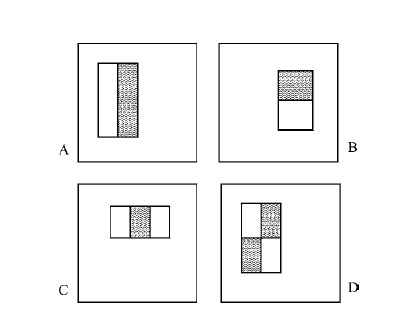
\includegraphics{ViolaJones} 
\caption{Two, three, and four feature rectangles used for facial detection in images.}\label{fig: 4}
\end{figure}
	
	
	
	 


\section{Neural Networks}
\begin{itemize}
\item What is a Neural Network?
\item Why are they used
\item layers, weights, and activation functions
\item Training and testing neural networks 
\item regularization techniques(not sure if this should go here)
\end{itemize}


\section{Back Propogation}
\begin{itemize}
\item What is back propogation?
\item How does back propogation help to train a Neural network?
\item Hyper parameters(Tuneable Parameters) and tuning them
\end{itemize}

\section{TensorFlow}
\begin{itemize}
\item What is tensorflow
\item what is a tensor
\item Using Tensorflow to build and train a neural network
\end{itemize}


\section{Convolutions}
\begin{itemize}
\item What is a convolution (or filter) ?
\item How are convolutions useful for image classification and computer vision?
\end{itemize}

\section{Convolutional Neural Networks}
\begin{itemize}
\item What happens in Biology when we look at things and try to identify them(Local receptive fields, etc.)
\item What is a convolutional layer?
\item What is a pooling layer/max pooling layer?
\item Building and training Convolutional Neural Networks with TensorFlow
\end{itemize}

\section{Image Classification Using Convolutional Neural Networks}
\begin{itemize}
\item How is Image classification done using convolutional neural networks?
\item storing and accessing images (database)
\item Using a pretrained CNN to classify an image as a label
\item Using the label to get a subset of photos in a database and (possibly) image to image classification using another convolutional neural network
\end{itemize}

\section{Implementation}
\begin{itemize}
\item What I did/used to solve this problem
\end{itemize}

\section{Results}
\begin{itemize}
\item What happened when I used, built and trained the convolutional neural networks to classify clothing items
\item How did my project do at classifying clothing items
\item Problems I encountered, how and why they occurred
\item Possible solutions to the problems I encountered
\end{itemize}

\section{Conclusions}
\begin{itemize}
\item Conclusions made about image classification for clothing using convolutional neural networks
\end{itemize}


%different bibliography styles can be found here: https://www.sharelatex.com/learn/Bibtex_bibliography_styles
\bibliographystyle{acm}

\bibliography{References}

\end{document}
